\chapter{Experiments with Biological Neural Tensors} 

\label{chapter-biological} 

\section{Data collection}

The neural spiking data (\cite{dyballa_manifold_2021}) were collected from lab experiments conducted on mice. The experimental setup is shown in the figure below. Visual stimuli of moving artificial gratings of six different types were flashed in front of the mouse. Each visual stimuli were moving in eight directions. Response of neurons in the mouse retina was recorded with electrodes and encoded in peristimulus (PSTH) diagrams. Each PSTH diagram shows the firing rate of one neuron over time for each of the eight directions respectively. Brighter pixels indicate higher firing rates.
\begin{figure}[H]
    \centering
        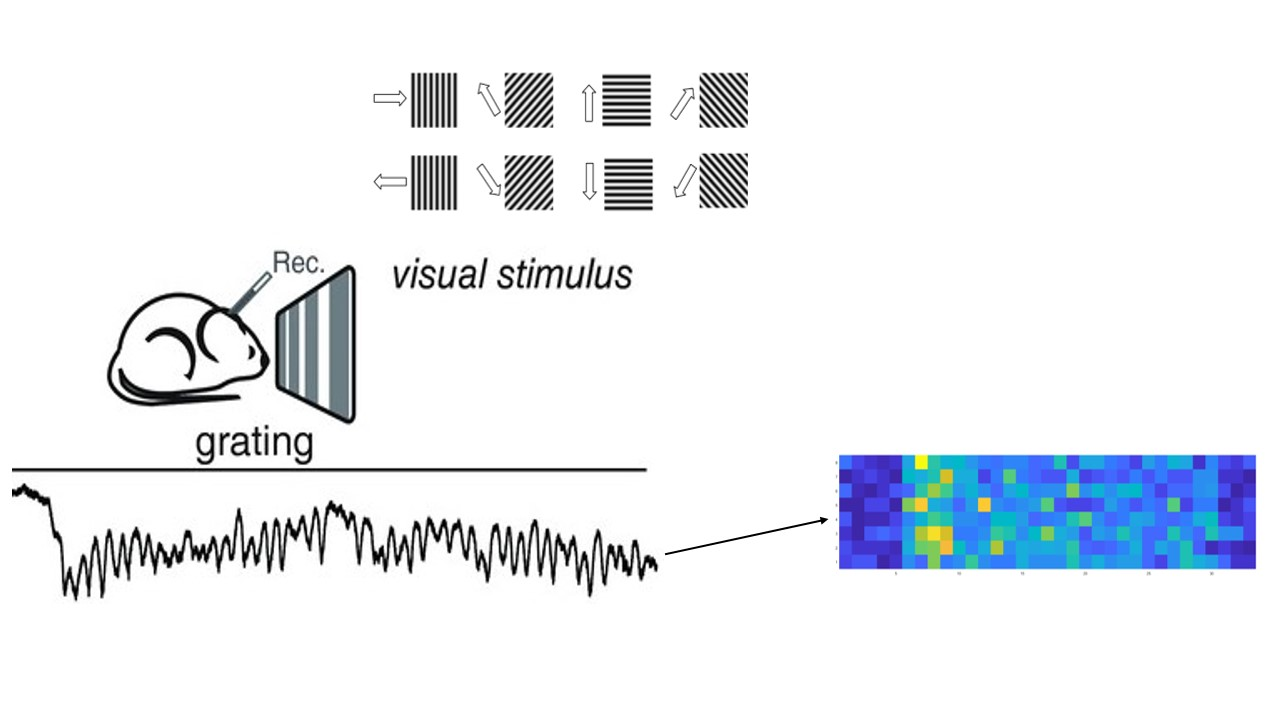
\includegraphics[width=0.6\textwidth]{presentation/Slide5.jpg}
        \caption{Visualising neural data from lab experiments.}
\end{figure}

\par The neural spiking data have $3$ dimensions: the first dimension represents the $698$ neurons, the second dimension represents the six different types of stimuli, and the third dimension represents represents the vectorized PSTH diagrams, each of which has $8\times 33 = 264$ pixels. Due to the number of dimensions, we need to generalize the familiar notion of matrix (which only has two dimensions) to its higher-order analogue, tensors, which we define as follows:

\begin{defn}[Tensors]
    An $N$-way tensor is an element of the tensor product of $N$ vector spaces. 
    
    A $1$-way tensor is a vector, $v = [v_1 \quad v_2 \quad \dots \quad v_n]^T.$ 
    
    A $2$-way tensor is a matrix, 
        $A = \left(\begin{matrix}
        A_{1 1} & A_{1 2} & \dots & A_{1 n}\\
        \vdots & \vdots & \vdots & \vdots \\ 
        A_{m 1} & A_{m 2} & \dots & A_{m n}
        \end{matrix}
        \right).$
    \end{defn}

\begin{defn}[Neural population response]
    Suppose $\mathcal{S}$ is a set of $S$ visual stimuli (e.g., images) $\mathcal{S} = \{s_1, s_2,\dots, s_S\}$, each moving over a time interval of $T$ in $d$ directions. The \underline{neural population response} of a set of $N$ neurons to a stimulus $m_i$ over time is $\mathcal{N} = \{\vec{n}_1, \vec{n}_2, \dots, \vec{n}_N\},$ where $\vec{n}_i \in \mathbb{R}^{dT}$. 
\end{defn}
\begin{defn}[Neural tensors]
    Each \underline{neural tensor} encodes the neural population response of a set of neurons to a set of moving visual stimulus over the time and directions of the movement. It is thus a $3$-way tensor of dimension $N$-by-$S$-by-$dT$.
\end{defn}

\section{Applying tensor CP decomposition}
To implement the tensor CP decomposition, we used the software, Tensor Toolbox for MATLAB. (\cite{tensortoolbox}) Our code is available in the GitHub repository\footnote{https://github.com/zhang-liu-official/capstone-liu-2022} for this project. After obtaining the tensor factors from tensor CP decomposition, we used PCA to project data onto a lower-dimensional linear subspace and k-means to label the clusters by distances in the lower-dimensional linear subspace. 

We can visualize the first five tensor factors from biological neural tensor:
    \begin{figure}[H]
        \centering
            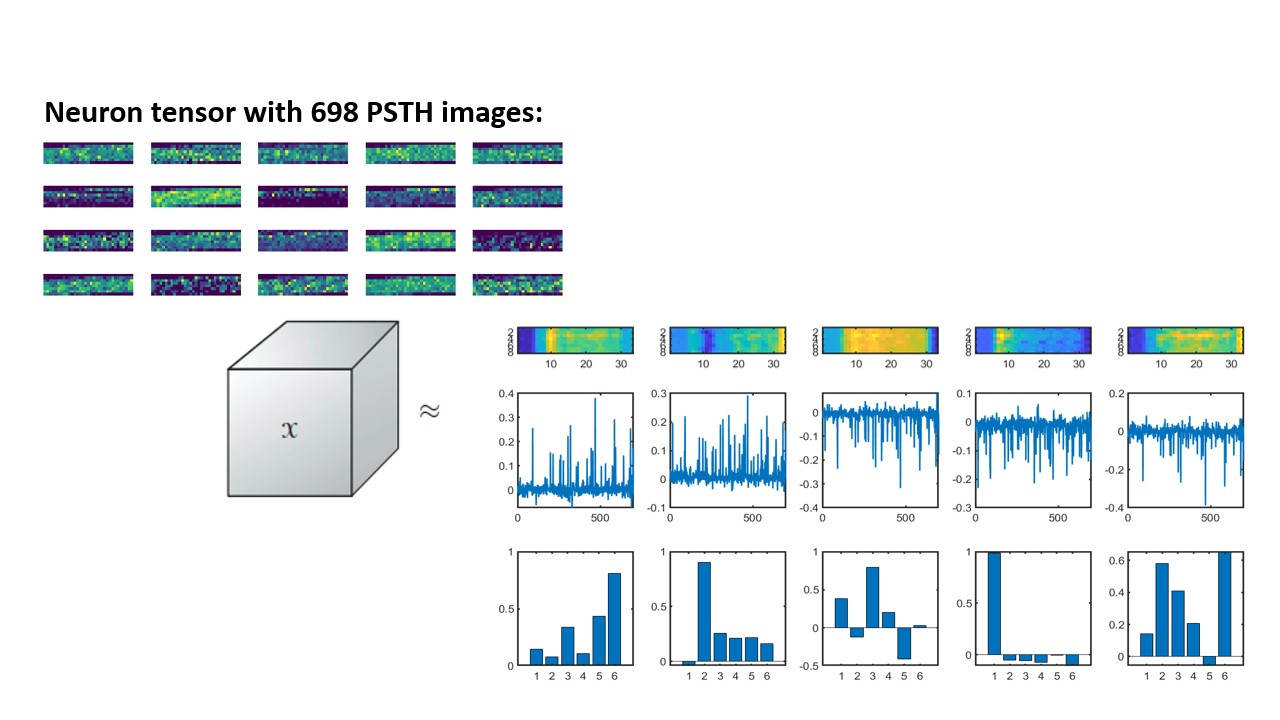
\includegraphics[width=\textwidth]{presentation/Slide3.jpg}
            \caption{First 5 tensor factors for neural data.}
        \end{figure} 

The neural manifold generated from the neural tensor shows the clusters of neurons grouped by their firing patterns encoded in the PSTH diagrams:
    \begin{figure}[H]
        \centering
            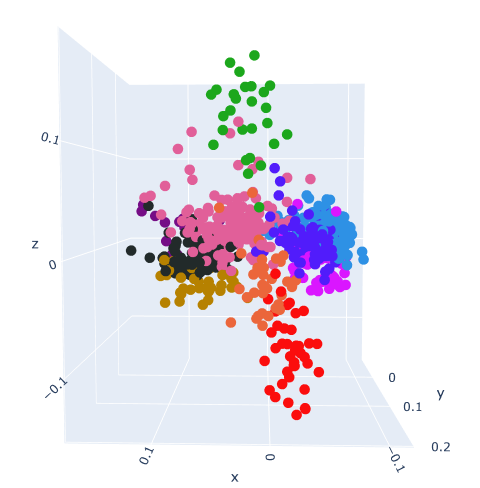
\includegraphics[width=\textwidth]{figures/embeddings/embedding-lab.png}
            \caption{Neural manifolds: clusters of neurons grouped by firing patterns, each point represent a neuron.}
        \end{figure} 

We can plot the PSTH diagrams associated with some points inside the neural manifold, where each point represents a neuron. 

      \begin{figure}[H]
            \centering
            \begin{subfigure}[b]{\textwidth}
                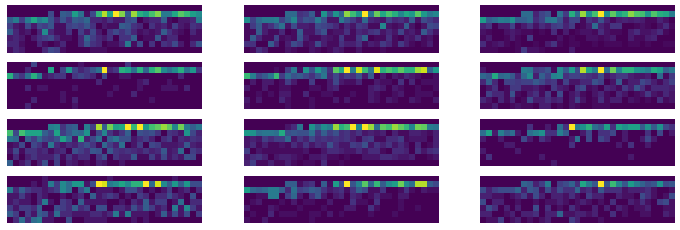
\includegraphics[width=0.95\textwidth]{presentation/figures-retina-results/cluster20.png}
                \caption{PSTH diagrams showing responses of neurons in an arbitrary cluster to stimulus type 1.}
            \end{subfigure}
            \vfill 
            \begin{subfigure}[b]{\textwidth}
                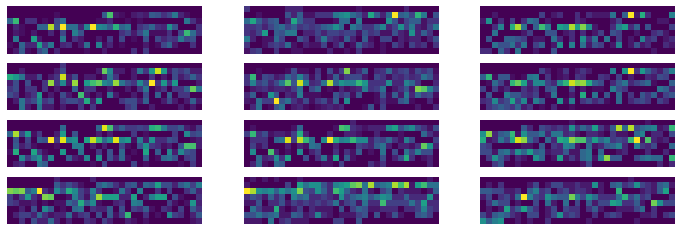
\includegraphics[width=0.95\textwidth]{presentation/figures-retina-results/cluster10.png}
                \caption{PSTH diagrams showing responses of neurons in another cluster to stimulus type 1.}
            \end{subfigure}
            \end{figure} 


\section{Applying diffusion map}
Recall that the neural spiking data set used in this project is represented by a $3$-way tensor of dimension $698$-by-$6$-by-$264$. The three dimensions represent neurons, stimuli, and firing patterns (PSTH diagram) respectively. With this neural spiking data set, we can create six point clouds, each corresponds to the neural population response towards one type of stimuli, which we denote as $X_1, X_2, \dots,X_6$. Each of the point cloud $X_i$ is thus represented by a matrix of dimension $698$-by-$264$, giving us a point cloud of $698$ points in $\RR^{264}$. 

We used the pydiffmap package (\cite{eastman_pydiffmap_2017}). In our implementation, we reduced the dimensionaltity of each point cloud from the space of $\RR^{264}$ to $\RR^3$ using diffusion map. The resulting three-dimensional embedding of the original point clouds colored by the first three diffusion coordinates are shown below:
\begin{figure}[H]
\centering
\begin{subfigure}[b]{0.3\textwidth}
    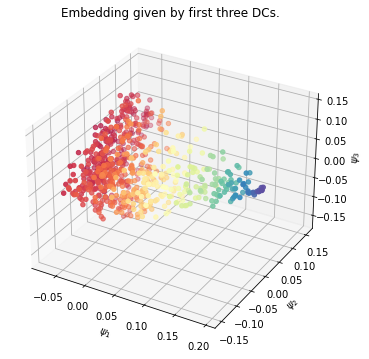
\includegraphics[width=\textwidth]{figures/topology/X1_embedding.png}
    \caption{Three-dimensional embedding of the original point cloud $X_1$.}
\end{subfigure}
\hfill
\begin{subfigure}[b]{0.3\textwidth}
    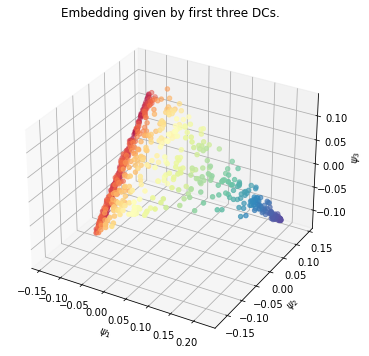
\includegraphics[width=\textwidth]{figures/topology/X2_embedding.png}
    \caption{Three-dimensional embedding of the original point cloud $X_2$.}
\end{subfigure}
\hfill
\begin{subfigure}[b]{0.3\textwidth}
    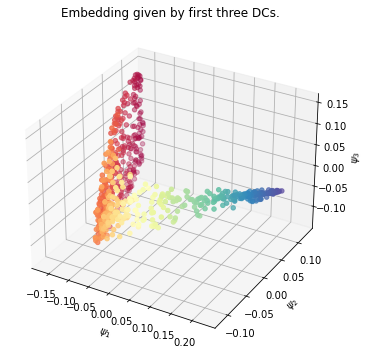
\includegraphics[width=\textwidth]{figures/topology/X3_embedding.png}
    \caption{Three-dimensional embedding of the original point cloud $X_3$.}
\end{subfigure}
\hfill
\begin{subfigure}[b]{0.3\textwidth}
    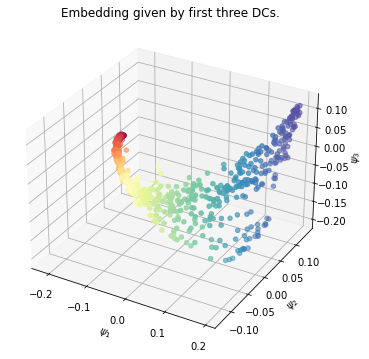
\includegraphics[width=\textwidth]{figures/topology/X4_embedding.png}
    \caption{Three-dimensional embedding of the original point cloud $X_4$.}
\end{subfigure}
\hfill
\begin{subfigure}[b]{0.3\textwidth}
    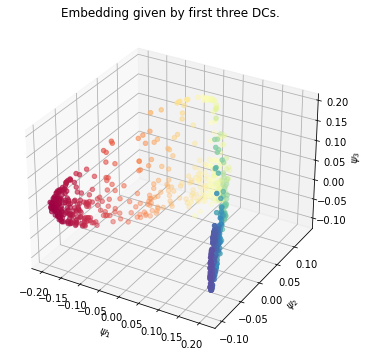
\includegraphics[width=\textwidth]{figures/topology/X5_embedding.png}
    \caption{Three-dimensional embedding of the original point cloud $X_5$.}
\end{subfigure}
\hfill
\begin{subfigure}[b]{0.3\textwidth}
    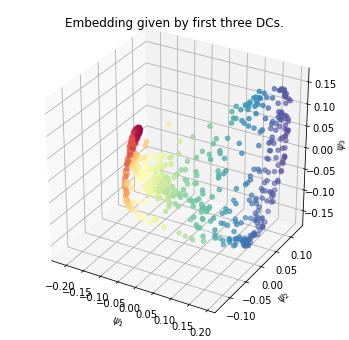
\includegraphics[width=\textwidth]{figures/topology/X6_embedding.png}
    \caption{Three-dimensional embedding of the original point cloud $X_6$.}
\end{subfigure}
\end{figure}
